\documentclass[11pt,reqno,twoside]{article}

%>>>>>>> DO NOT EDIT MACRO FILE




% >>>> DO NOT EDIT THIS FILE
% If you *must* add or change a macro, please email mccoy@caltech.edu

%=================================================
% Basics
%=================================================

\usepackage{fixltx2e} % Makes \( \) equation style robust, among other
                      % things. Must be the first package.


% Makes ligatured fonts searchable and copyable in pdf readers
\usepackage{cmap} % Load before fontenc 

% Always include these font encodings in your document 
% unless you have a very good reason.
\usepackage[T1]{fontenc}
\usepackage[utf8]{inputenc}
\usepackage{graphicx}
\usepackage{placeins}
\usepackage{enumerate}
\usepackage{algcompatible}

\usepackage{verbatim}




%=====================================
% Look & feel
%=====================================

% Allows for manual space setting
\usepackage{setspace}

%=============
% Fonts
%=============
\let\counterwithout\relax     %DSA: i had to include this to be able to compile
\let\counterwithin\relax  %DSA: i had to include this to be able to compile
\usepackage{lmodern} % Improved version of computer modern
\usepackage[scale=0.88]{tgheros} % Helvetica clone for sans serif font


\newcommand\hmmax{2} % Default is 3.
\newcommand\bmmax{2} % Default is 4.

\usepackage{bm} % boldmath must be called after the package
\providecommand{\mathbold}[1]{\bm{#1}}

\usepackage{bbold}



%=============
% AMS Packages and fonts
%=============
\usepackage{amsmath,amsbsy,amsgen,amscd,amsthm,amsfonts,amssymb} 

%=============
% Margins and paper size
%=============
\usepackage[centering,top=1.5in,bottom=1.2in,left=1.4in,right=1.4in]{geometry}

%=============
% Title setup
%=============
\usepackage{titling}
\usepackage{musicography}
%\usepackage{nopageno}
\setlength{\droptitle}{-7.5em}


%=============
% Section headings
%=============
\usepackage[sf,bf,compact]{titlesec}

%=============
% Tables and lists
%=============
\usepackage{booktabs,longtable,tabu} % Nice tables
\setlength{\tabulinesep}{1mm}
\usepackage[font=small,margin=12pt,labelfont={sf,bf},labelsep={space}]{caption}


%\usepackage{enumitem}
%\setitemize{itemsep=0pt} 
%\setenumerate{itemsep=0pt}
%\setlist[1]{labelindent=\parindent,% % Recommended by enumitem package
% }
% 
% 


%=============
% Hyperlink colors
%=============
\usepackage[usenames,dvipsnames]{xcolor}

\definecolor{dark-gray}{gray}{0.3}
\definecolor{dkgray}{rgb}{.4,.4,.4}
\definecolor{dkblue}{rgb}{0,0,.5}
\definecolor{medblue}{rgb}{0,0,.75}
\definecolor{rust}{rgb}{0.5,0.1,0.1}

\usepackage{url}
\usepackage[colorlinks=true]{hyperref}
\hypersetup{linkcolor=dkblue}    
\hypersetup{citecolor=rust}      
\hypersetup{urlcolor=rust}     

%=============
% Microtype
%=============
\usepackage[final]{microtype} 

%=============
% 

%=============
\newtheoremstyle{myThm} % name
    {\topsep}                    % Space above
    {\topsep}                    % Space below
    {\itshape}                   % Body font
    {}                           % Indent amount
    {\sffamily\bfseries}                   % Theorem head font
    {.}                          % Punctuation after theorem head
    {.5em}                       % Space after theorem head
    {}  % Theorem head spec (can be left empty, meaning ‘normal’)

\newtheoremstyle{myRem} % name
    {\topsep}                    % Space above
    {\topsep}                    % Space below
    {}                   % Body font
    {}                           % Indent amount
    {\sffamily}                   % Theorem head font
    {.}                          % Punctuation after theorem head
    {.5em}                       % Space after theorem head
    {}  % Theorem head spec (can be left empty, meaning ‘normal’)

\newtheoremstyle{myDef} % name
    {\topsep}                    % Space above
    {\topsep}                    % Space below
    {}                   % Body font
    {}                           % Indent amount
    {\sffamily\bfseries}                   % Theorem head font
    {.}                          % Punctuation after theorem head
    {.5em}                       % Space after theorem head
    {}  % Theorem head spec (can be left empty, meaning ‘normal’)

\theoremstyle{myThm}
\newtheorem{theorem}{Theorem}[section]
\newtheorem{lemma}[theorem]{Lemma}
\newtheorem{proposition}[theorem]{Proposition}
\newtheorem{corollary}[theorem]{Corollary}
\newtheorem{fact}[theorem]{Fact}
\newtheorem{assumption}[theorem]{Assumption}

\theoremstyle{myRem}
\newtheorem{remark}[theorem]{Remark}

\theoremstyle{myDef}
\newtheorem{definition}[theorem]{Definition}
 \newtheorem{example}[theorem]{Example}

%=====================
% Header
%=====================
\usepackage{fancyhdr}
\usepackage{nopageno} % Gets rid of page number at the bottom
\fancyhf{} % Clear header style
\renewcommand{\headrulewidth}{0.5pt} % remove the header rule
\pagestyle{fancy}
\fancyhead[LE,RO]{\textsf{\small \thepage}}

\setlength{\headheight}{14pt}
%=====================
% Fix delimiters
%=====================

% Fixes \left and \right spacing issues. See discussion at
% http://tex.stackexchange.com/questions/2607/spacing-around-left-and-right
\let\originalleft\left
\let\originalright\right
\renewcommand{\left}{\mathopen{}\mathclose\bgroup\originalleft}
\renewcommand{\right}{\aftergroup\egroup\originalright}




%=================================================
% Math macros
%=================================================

%=============
% Generalities
%=============
\usepackage{mathtools}
\mathtoolsset{centercolon}  % Makes := typeset correctly for definitions


%%% Equation numbering
%\numberwithin{equation}{section} 

%%% Annotations
\newcommand{\notate}[1]{\textcolor{red}{\textbf{[#1]}}}

%==============
% Symbols
%==============
\let\oldphi\phi
\renewcommand{\phi}{\varphi}
\newcommand{\eps}{\varepsilon}

%==============
% Constants
%==============

% Set constants upright
\newcommand{\cnst}[1]{\mathrm{#1}}  
\newcommand{\econst}{\mathrm{e}}

\newcommand{\zerovct}{\vct{0}} % Zero vector
\newcommand{\Id}{{I}} % Identity matrix
\newcommand{\onemtx}{\bm{1}}
\newcommand{\zeromtx}{\bm{0}}

%==============
% Sets
%==============
\providecommand{\mathbbm}{\mathbb} % In case we don't load bbm

% Reals, complex, naturals
\newcommand{\R}{\mathbbm{R}}
\newcommand{\C}{\mathbbm{C}}
\newcommand{\N}{\mathbbm{N}}
\newcommand{\Z}{\mathbbm{Z}}
\newcommand{\la}{\langle}
\newcommand{\ra}{\rangle}


%=======
%Colors
%=======
\newcommand{\red}{\color{red}}
\newcommand{\blue}{\color{blue}}
\definecolor{mygreen}{rgb}{0.1,0.75,0.2}
\newcommand{\grn}{\color{mygreen}}
\newcommand{\nc}{\normalcolor}


%==============
% Basics
%==============
\newcommand{\pr}{f}
\newcommand{\post}{\pi}
\newcommand{\like}{L}
\newcommand{\noise}{\nu}
\newcommand{\loss}{\mathsf{L}}
\newcommand{\reg}{\mathsf{R}}
\newcommand{\precision}{\Omega}
\newcommand{\Y}{Y}
\newcommand{\X}{\mathbb{X}}
\newcommand{\varg}{v}

%%%%%
%Prior and posterior means and covariances
\newcommand{\mpr}{\hat{m}}
\newcommand{\mpost}{m}
\newcommand{\Cpr}{C}
\newcommand{\Cpost}{C}


\newcommand{\bmu}{{\boldsymbol{\mu}}}

%==============
% Probability
%==============
\newcommand{\Prob}{\operatorname{\mathbbm{P}}}
\newcommand{\Expect}{\operatorname{\mathbb{E}}}
\newcommand{\V}{\operatorname{\mathbb{V}}}
\newcommand{\Sam}{N}
\newcommand{\sam}{n}
\newcommand{\pdfs}{{\mathscr{P}}}


%==============
% Dimensions
%==============
\newcommand{\Du}{d}
\newcommand{\du}{i}
\newcommand{\Dy}{k}
\newcommand{\dy}{i}
\newcommand{\Ru}{\mathbbm{R}^\Du}
\newcommand{\Ry}{\mathbbm{R}^\Dy}

%==============
% Vectors and matrices 
%==============
\newcommand{\vct}[1]{{#1}}
\newcommand{\mtx}[1]{{#1}}

%%%%%%%%%%%%%
\newcommand{\umap}{u_{\mbox {\tiny{\rm MAP}}}}
\newcommand{\upm}{u_{\mbox {\tiny{\rm PM}}}}


\newcommand{\prwmh}{p_{\mbox {\tiny{\rm RWMH}}}}
\newcommand{\qrwmh}{q_{\mbox {\tiny{\rm RWMH}}}}
\newcommand{\pind}{p_{\mbox {\tiny{\rm ind}}}}
\newcommand{\ppcn}{p_{\mbox {\tiny{\rm pCN}}}}
\newcommand{\pmh}{p_{\mbox {\tiny{\rm MH}}}}
\newcommand{\pdugs}{p_{\mbox {\tiny{\rm DUGS}}}}
\newcommand{\qlgv}{q_{\mbox {\tiny{\rm Lgv}}}}
\newcommand{\qpcn}{q_{\mbox {\tiny{\rm pCN}}}}
\newcommand{\qind}{q_{\mbox {\tiny{\rm ind}}}}
\newcommand{\pgs}{p_{\mbox {\tiny{\rm GS}}}}


% Metrics between probability measures
\newcommand{\dkl}{d_{\mbox {\tiny{\rm KL}}}}
\newcommand{\dwas}{d_{\mbox {\tiny{\rm W}}}}
\newcommand{\dwasp}{d_{\mbox {\tiny${\rm W}_p$}}}
\newcommand{\dtv}{d_{\mbox {\tiny{\rm TV}}}}
\newcommand{\dchi}{d_{\mbox {\tiny{$ \chi^2$}}}}
\newcommand{\dhell}{d_{\mbox {\tiny{\rm H}}}}
\newcommand{\Nc}{\mathcal{N}}

\usepackage[]{algorithm}

\usepackage{graphicx, subfig}


\usepackage{authblk}
\usepackage[square,numbers]{natbib}
\makeatletter
\makeatother
\usepackage{chngcntr}
\usepackage{mathrsfs}
\counterwithin{table}{section}
\counterwithin{algorithm}{section}
%\usepackage{draftwatermark}
%\SetWatermarkText{DRAFT}
%\SetWatermarkScale{1}

\title{\Huge{Monte Carlo Simulation} \\
\huge{X-Page Essay}} % CORRECT TITLE
% TIP:  Use "\\" to break the title into more than one line.
\author{ \Large{Your Name }\\
Department of Statistics, University of Chicago}


\vspace{.25in} 

\date{}
%>>>>>>> NAME OF SCRIBE(S) AND EDITOR(S)
%\author{%
  %Scribe:& 
  %Group Names  % >>>>> SCRIBE NAME(S)
%}

\makeatletter\@addtoreset{section}{part}\makeatother%
\numberwithin{equation}{section}


\renewcommand{\triangleq}{:=}
\newcommand{\upperRomannumeral}[1]{\uppercase\expandafter{\romannumeral#1}}
\newcommand{\lowerromannumeral}[1]{\romannumeral#1\relax}
\renewcommand{\hat}{\widehat}

%Precision and analysis operators
\newcommand{\An}{{\mathcal{A}}}
\newcommand{\Pred}{{\mathcal{P}}}

%Objective functionals
\newcommand{\J}{{\mathsf{J}}}
\newcommand{\I}{{\mathsf{I}}}
\newcommand{\JJ}{{\mathcal{J}}}

\begin{document}
\maketitle %  LEAVE HERE
% The command above causes the title to be displayed.

%>>>>> DELETE ALL CONTENT UNTIL "\end{document}"
% This is the body of your document.




 \newpage \section{\Large{\sffamily{Title}}}

\red This is a template so you don't have to waste time looking up environments for the algorithms, sections, theorems, figures, examples etc.  Please use this template for your essays. The cover page doesn't count for the page limit. \nc

\subsection{Transformation Methods}\label{ssec:transformation}
Given a random variable $X: \Omega \rightarrow E \subseteq \R$, we seek to find a deterministic function $\phi$ such that
$$X=\phi(U),$$
where here and below $U\sim \text{Unif}(0,1)$ and equality is interpreted in distribution. Once such $\phi$ is found, a sample from $f_X$ can be obtained as follows.


\FloatBarrier
\begin{algorithm}
\caption{General transformation method}
\begin{algorithmic}[1]
\STATE {\bf Input}: Transformation $\phi$ such that $X = \phi(U).$
\STATE Set $X^{(n)}=\phi(U^{(n)}),\quad 1\leq n\leq N,$ \quad 
where $U^{(n)}\stackrel{\text{i.i.d.}}{\sim} \text{Unif}(0,1)$.\STATE {\bf Output}: $X^{(n)}\stackrel{\text{i.i.d.}}{\sim}f_X.$
\end{algorithmic}
\end{algorithm}

 


\subsubsection{Inverse Transformation Method}\label{sssec:inversetransformation}
Given a real-valued random variable $X$, the inverse tranformation method is a general way to find $\phi$ with $X = \phi(U).$ It is defined in terms of the CDF $F_X$ of the variable $X.$

\begin{theorem}[Inverse Tranformation Method]\label{thm:inversetransf}
Define $\phi (u):= \inf\{x:F_X(x)\geq u\}\equiv F_X^-(u)$. If $U\sim \emph{Unif}(0,1)$, then $F_X^-(U)=X.$
\end{theorem}
\begin{proof}
We only prove here the case where $F_X$ is a bijection from $(-\infty,\infty)$ to $(0,1).$ In such a case $F_X^-=F_X^{-1}$, see Figure \ref{fig:transformationmethod}.
Then
$$\Prob \bigl(F_X^-(U)\leq x\bigr)=\Prob \bigl(F_X^{-1}(U)\leq x\bigr)=\Prob\bigl(U\leq F_X(x)\bigr)=F_X(x),$$
which shows that the CDF of the random variable $F_X^-(U)$ is $F_X$.
\end{proof}


\begin{remark}
The inverse transform method is simply Algorithm 1 with the choice $\phi (U) : = F_X^-(U)$.
\end{remark}

\noindent
\ \textbf{Advantages of the Inverse Transformation Method}
\vspace{-0.25cm}
\begin{itemize}
\item It is efficient if $F_X^-$ has a closed form expression that can be evaluated cheaply.
\end{itemize}
\noindent
\ \textbf{Disadvantages of the Inverse Transformation Method}
\vspace{-0.25cm}
\begin{itemize}
\item Typically $F_X^-$ does not have a closed form expression that is easy to evaluate.
\vspace{-0.2cm}
\item It is a dead-end: it is not clear how to generalize the method to high dimensional problems where $X$ takes values in $\R^d,$ $d>1,$ even though in some cases it may be possible.
\end{itemize}

  \FloatBarrier
    \begin{figure}[htp]
      \centering
      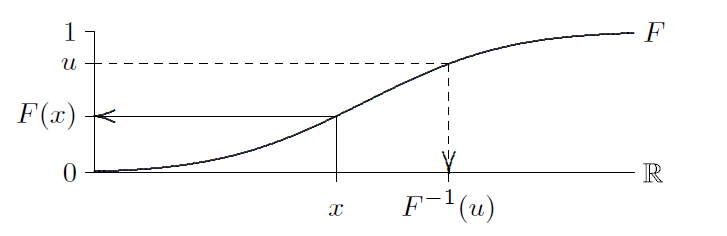
\includegraphics[width=0.75\columnwidth]{transformationmethod.png}
      \caption{A strictly increasing CDF and associated inverse CDF.}
      \label{fig:transformationmethod}
    \end{figure}
    \FloatBarrier



\subsubsection{Other Transformation Methods}\label{sssec:othertransformations}
The inverse transformation method is only one choice of transformation $\phi$ such that $X=\phi(U)$ and in our presentation above is restricted to real-valued variables. Other transformation methods may be applied and their use needs not be restricted to the one-dimensional setting. A classical example is the Box Muller method, which allows to obtain samples $X^{(1)},X^{(2)} \stackrel{\text{i.i.d.}}{\sim} \Nc(0,1)$ (that may be seen as one sample from a bivariate normal dsitribution) from samples $U^{(1)},U^{(2)} \stackrel{\text{i.i.d.}}{\sim} \text{Unif}(0,1)$.

\begin{example}{(Box Muller Method.)} \\
Suppose $X_1,X_2 \stackrel{\text{i.i.d.}}{\sim} \Nc(0,1)$, and write
\begin{align*}
X_1&=R\cos\theta,\\
X_2&=R\sin\theta,\\
\theta &\in [0,2\pi).
\end{align*}
Then blablabla
\end{example}







\subsection{Discussion and Bibliography}

Transformation methods and accept-reject methods can be found in virtually any textbook on Monte Carlo methods, see e.g.  \cite{robert2013monte}. 









\newpage
\newpage

\newpage
\bibliographystyle{abbrvnat} 

\bibliography{references}



\end{document}